\begin{frame}
\frametitle{About This Work...}

\emph{Scalable Continuous Range Monitoring of Moving Objects in Symbolic Indoor Space}.~\cite{DBLP:conf/cikm/YangLJ09} \\
B.~Yang, H.~Lu, and C.~S. Jensen.\\~\\

\begin{itemize}
  \item Published in \emph{CIKM' 2009}.
  \item Application: continuously monitor indoor moving objects for space use analysis or security purposes.
  \item An incremental, query-aware continuous range query processing technique for objects moving in indoor space.
  \item Use maximum speed constraint on object movement to refine the uncertain results.
\end{itemize}

\end{frame}
%------------------------------------------------

\begin{frame}
\frametitle{Motivation}

\begin{itemize}
  \item People spend much time in indoor spaces.

  \item Indoor spaces are becoming increasingly larger and complex.
    \begin{itemize}
      \item E.g., London Underground, 268 stations, 408 kilometers of network, +4 million daily passengers.
    \end{itemize}

  \item Indoor monitoring of people can help support.
    \begin{itemize}
      \item space use analysis
      \item security purposes
    \end{itemize}
\end{itemize}

\end{frame}

%------------------------------------------------

\begin{frame}
\frametitle{Preliminaries: Indoors vs. Outdoors}

\begin{itemize}
  \item Modeling of indoor spaces do not assume~\cite{jensen2010indoor}
    \begin{itemize}
      \item Euclidean space. (since obstacles render movement more constrained)
      \item Spatial network. (since indoor movement is less constrained than movements in polylines)
    \end{itemize}

  \item Instead indoor spaces are characterized by entities~\cite{DBLP:conf/mdm/JensenLY09}.
    \begin{itemize}
      \item Doors, rooms, hallways, staircase, etc.
    \end{itemize}

  \item \conceptbf{Symbolic models} are more suitable~\cite{becker2005location}.

  \item \emph{GPS} and \emph{cellular tracking} do not work indoors.

  \item Sensing devices are used to detect objects within their activation range, e.g., RFID readers or Bluetooth hotspots.
\end{itemize}

\end{frame}

%------------------------------------------------

\begin{frame}
\frametitle{Positioning Devices Deployment Graph}

\begin{columns}[c]

  \column{.57\textwidth}
  \begin{itemize}
    \fsize{
    %\item More advanced compared to \emph{RFID Deployment Graph}.
    \item Two types of positioning devices
      \begin{itemize}
        \ssize{
        \item Partitioning Device -- \emph{undirected} (\conceptbf{UP}), e.g., $d_{21}$ -- \emph{directed} (\conceptbf{DP}), e.g., $d_{11}$ and $d_{11'}$
        \item Presence Device -- (\conceptbf{PR})
        }
      \end{itemize}
    \item Note an indoor space is partitioned into \emph{activation ranges} and \emph{cells}
    }
  \end{itemize}
  \begin{block}{Deployment Graph}
    \textrm{
    \begin{itemize}
      \ssize{
      \item $G = \{C, E, \Sigma_{devices}, l_E\}$
      \item $C$: the set of cells
      \item $E$: the set of edges, $\{ c_i, c_j \}$ where $c_i, c_j \in C$
      \item $\Sigma_{devices}$: a mapping from $deviceID$ to activation range and type
      \item $l_E$ maps an edge to a set of positioning devices, i.e., $E \rightarrow 2^{\Sigma_{devices}}$
      }
    \end{itemize}
    }
  \end{block}

  \column{.43\textwidth}
    \vspace{-30pt}
    \begin{figure}[tb]
      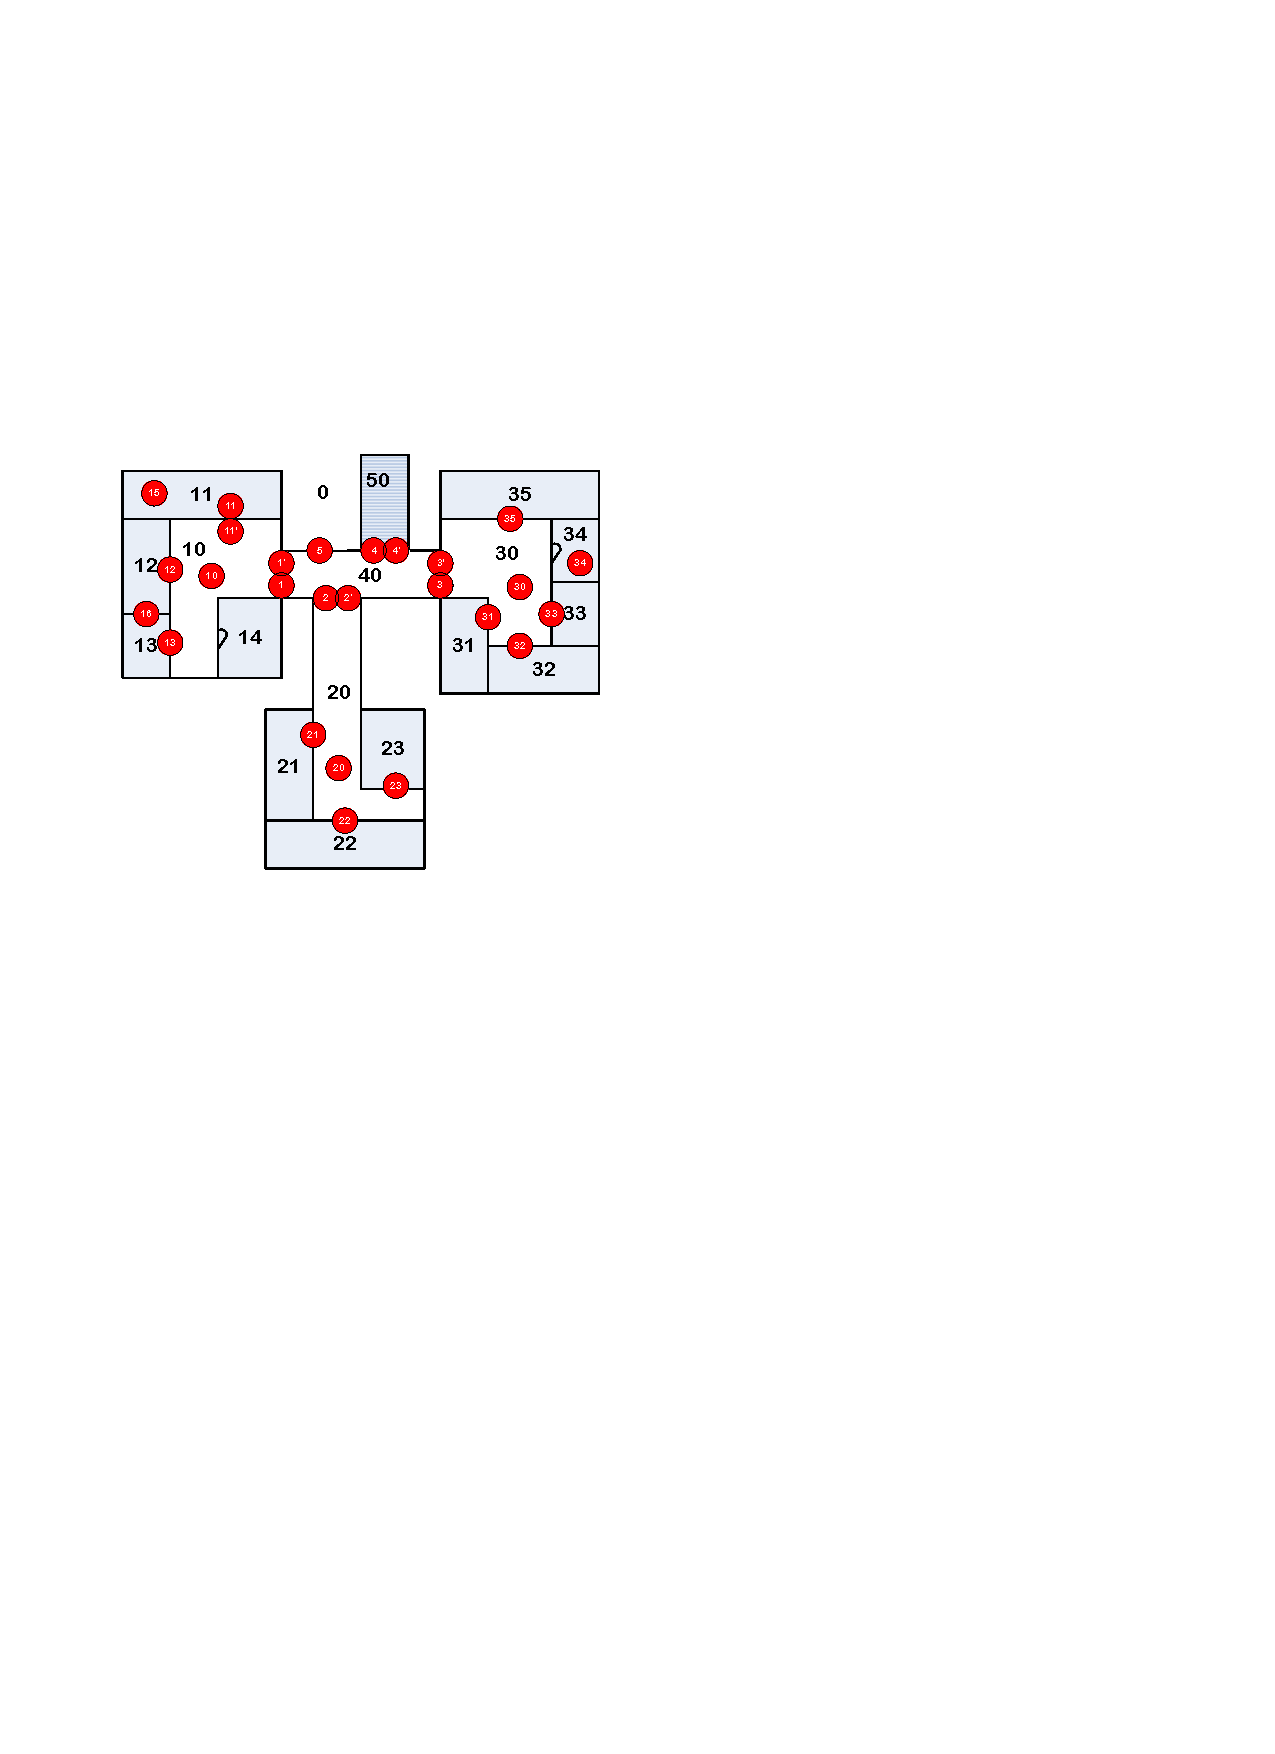
\includegraphics[width=\columnwidth]{figures/2-2/2-2-1.pdf}
    \end{figure}
    \vspace{-20pt}
    \pause
    \begin{figure}[tb]
      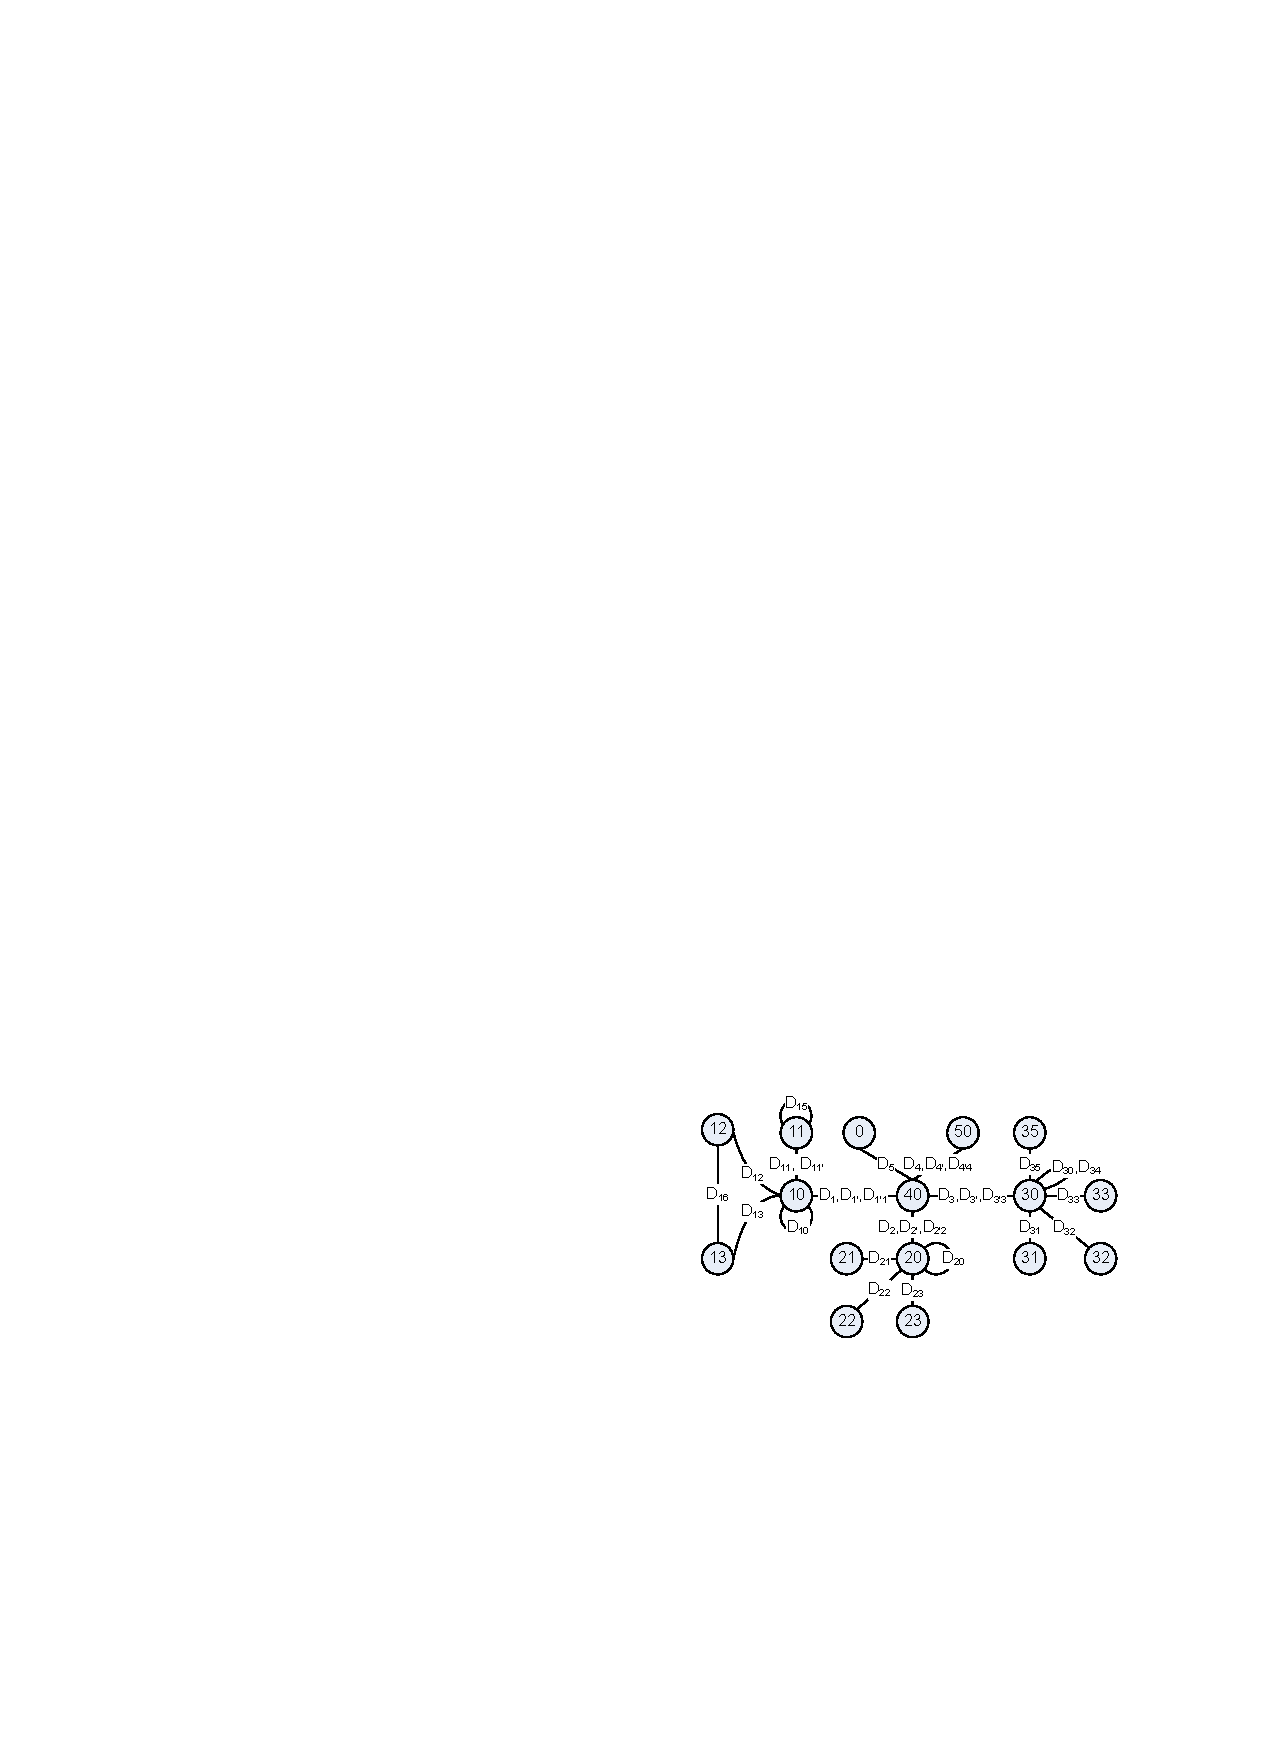
\includegraphics[width=\columnwidth]{figures/2-2/2-2-2.pdf}
    \end{figure}

\end{columns}

\end{frame}

%------------------------------------------------

\begin{frame}
\frametitle{States of Indoor Moving Objects}

%\begin{columns}[c]

  %\column{.57\textwidth}
  \begin{figure}[tb]
    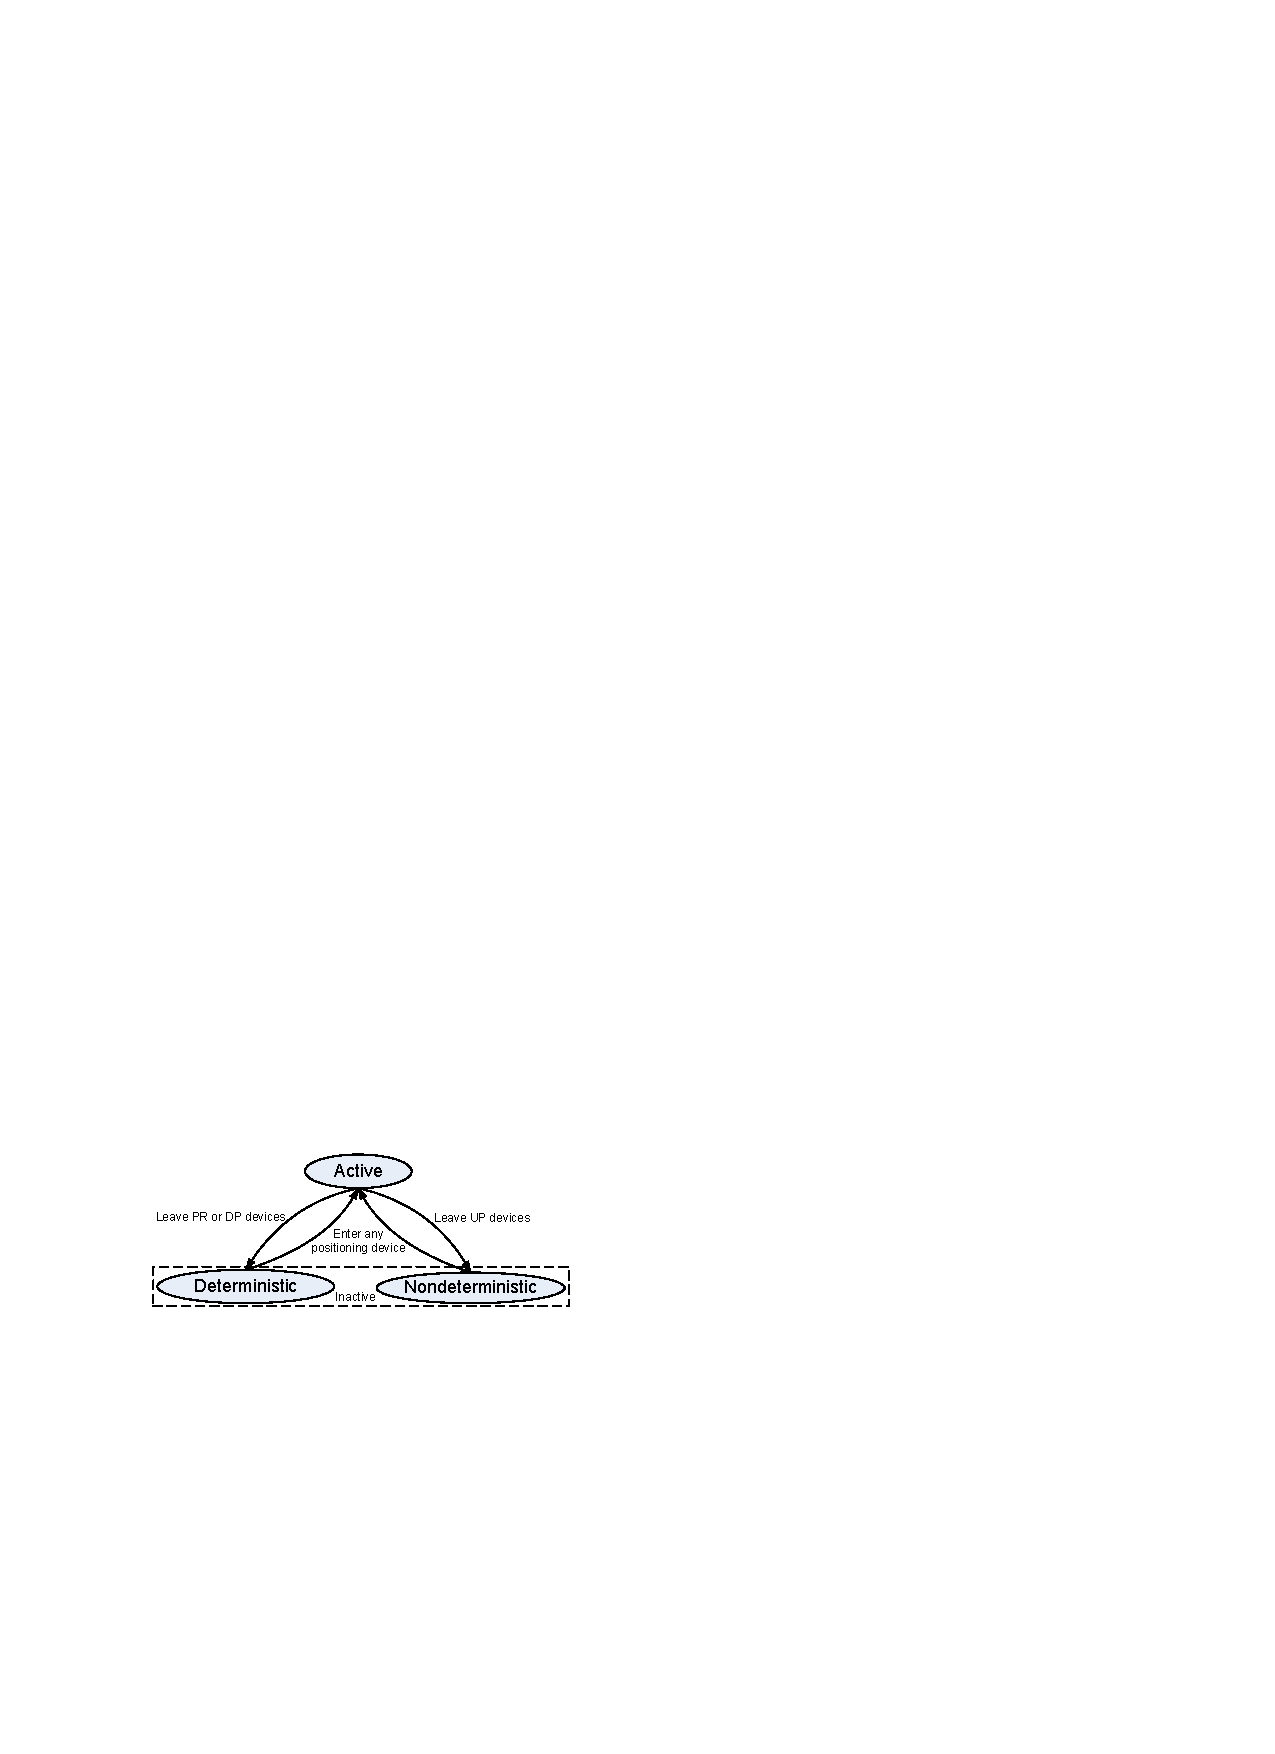
\includegraphics[width=0.6\columnwidth]{figures/2-2/2-2-3.pdf}
  \end{figure}
  \vspace{-10pt}
  %\column{.43\textwidth}
  \begin{itemize}
    \item An object is in an \conceptbf{active state} when it is inside the activation range of a positioning device.
    \item Otherwise the object is in an \conceptbf{inactive state}
    \item When an object is in the inactive state it is
      \begin{itemize}
        \item \conceptbf{nondeterministic} if it can be in more than one cell
        \item \conceptbf{deterministic} if it is in one specific cell
      \end{itemize}
  \end{itemize}

%\end{columns}

\end{frame}

%------------------------------------------------

\begin{frame}
\frametitle{Indexing Indoor Moving Objects}

\conceptbf{The proposed indexing scheme uses 4 hash tables}
\\~\\
\pause

\fsize{
\emph{Device Hash Table(DHT)} maps each device to a set of active objects:
\pause
$$DHT[deviceID] = O_A;~deviceID \in \Sigma_{devices}, O_A \subseteq O_{indoor}$$
\\~\\
\pause

\emph{Cell Deterministic Hash Table(CDHT)} maps each cell to a set of deterministic objects:
\pause
$$CDHT[cellID] = O_D;~cellID \in C, O_D \subseteq O_{indoor}$$
\\~\\
\pause

\emph{Cell Nondeterministic Hash Table(CNHT)} maps each cell to a set of nondeterministic objects:
\pause
$$CNHT[cellID] = O_N;~cellID \in C, O_N \subseteq O_{indoor}$$
\\~\\
\pause

\emph{Object Hash Table(OHT)} maps objects to their current data(state, time, cell(s) the object can be in)
\pause
$$OHT[objectID] = (STATE, t, IDSet);~objectID \in O_{indoor}$$
\\~\\
\pause
}

\end{frame}

%------------------------------------------------

\begin{frame}
\frametitle{RFID Deployment Graph Construction}

\begin{columns}[c]

  \column{.47\textwidth}
    \begin{figure}[tb]
      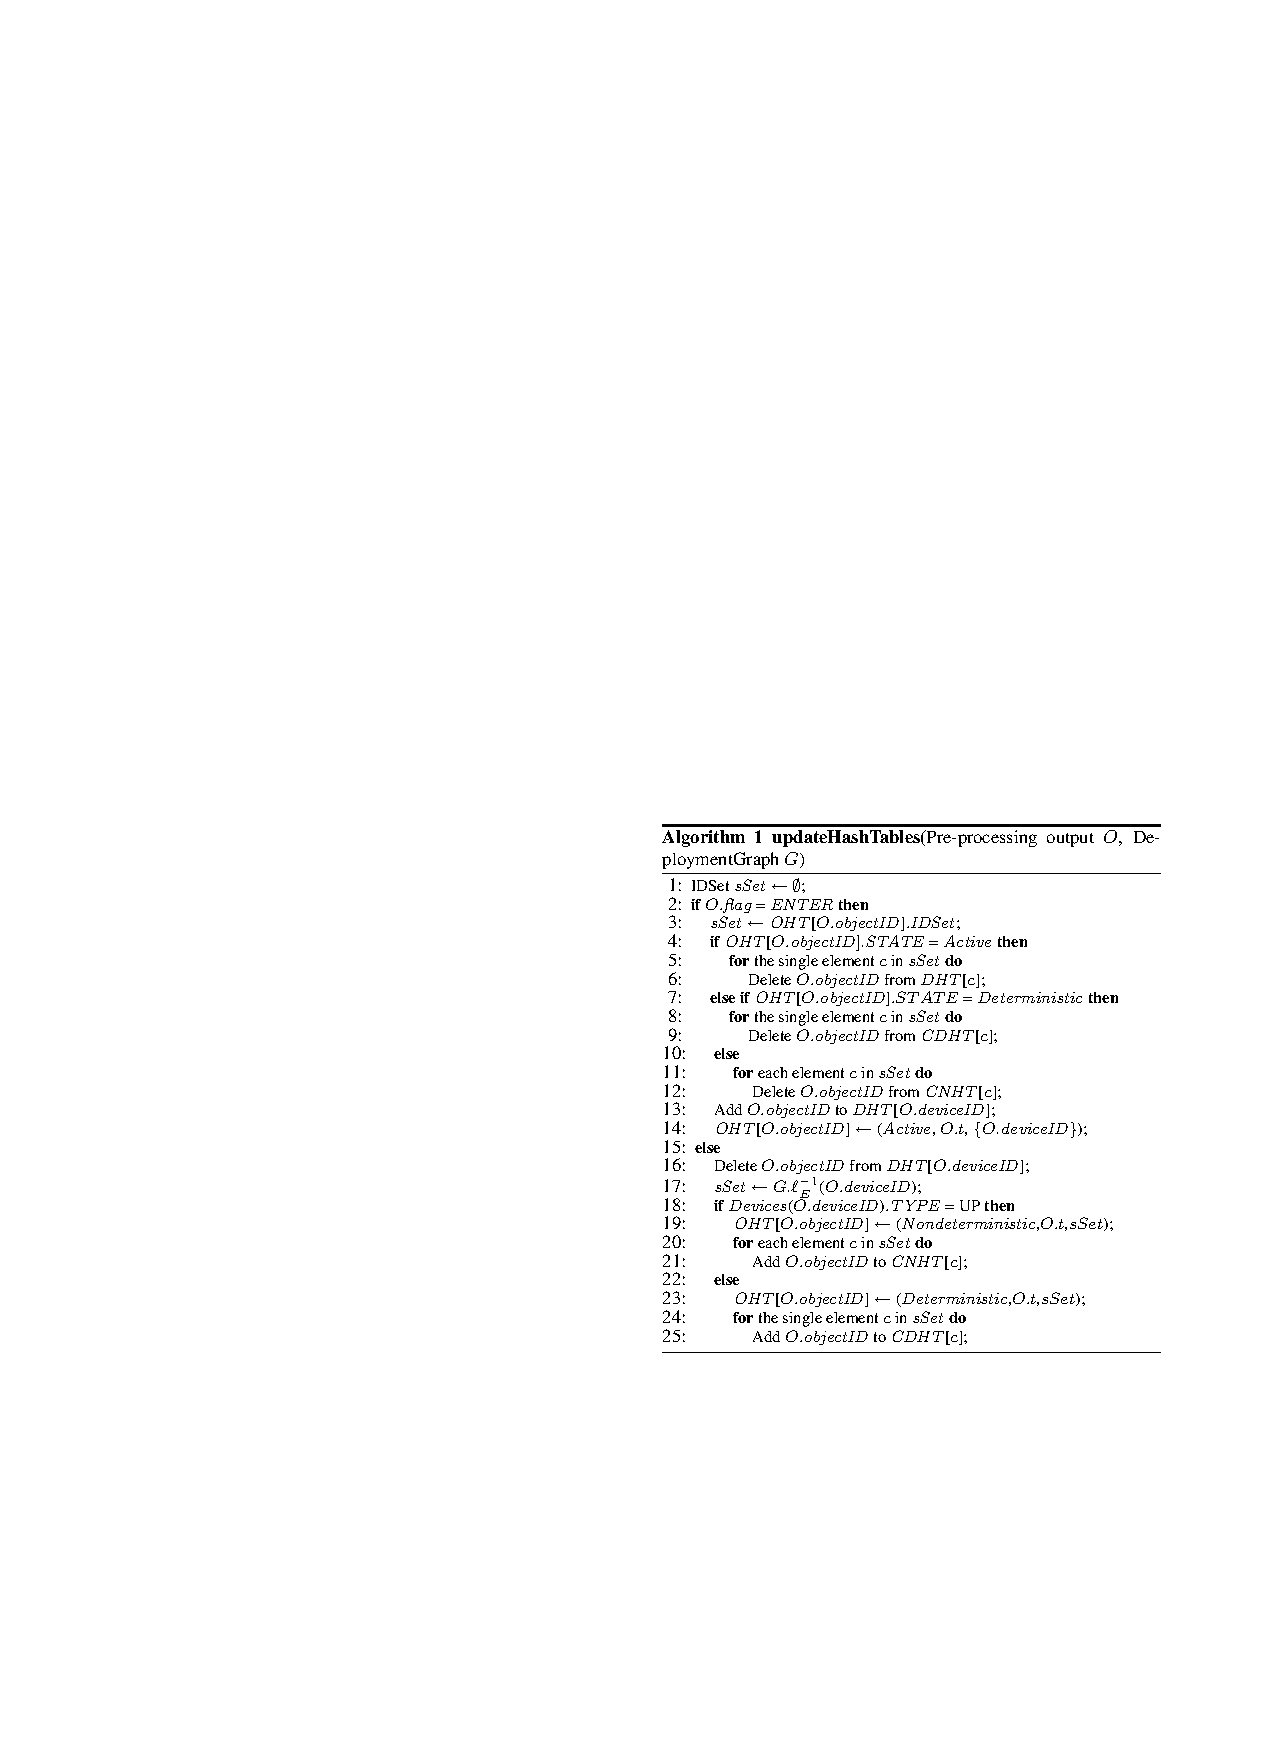
\includegraphics[width=\columnwidth]{figures/2-2/2-2-4.pdf}
    \end{figure}

  \column{.53\textwidth}
  \ssize{
    \begin{enumerate}
      \pause
      \item Line 1: \textrm{reset $IDSet$} \pause
      \item Lines 2--12: \textrm{$O.flag$ is ENTER so check the object's previous state. Remove $O$ from the corresponding table according its previous state} \pause
      \item Lines 13--14: \textrm{add $O$ to table of active objects (DHT), and update $O$'s in the objects' table (OHT)} \pause
      \item Lines 16--17: \textrm{$O.flag$ is LEAVE so remove the object from DHT. Get the possible cells that $O$ can move to} \pause
      \item Lines 18--25: \textrm{if the device is undirected, set $O$ in OHT and add $O$ to CNHT for the cells in sSet, else apply the same to CDHT}
    \end{enumerate}
  }
  \end{columns}

\end{frame}

%------------------------------------------------

\begin{frame}
\frametitle{Continuous Range Monitoring: Query Definition}

\begin{itemize}
  \item A \emph{Continuous Range Monitoring Query} (CRMQ)
    \begin{itemize}
      \item takes an \conceptbf{indoor spatial range} $\bf R$ as parameter
      \item keeps reporting the objects when it is registered for a certain time frame $[t_s, t_e]$
    \end{itemize}
  \item The \conceptbf{query result} $\bf \mathcal{M}$ -- the set of moving objects in $\bf R$ - is maintained as follows:
    \begin{equation*}
      \forall t \in [t_s, t_e]: o \in CRMQ[R](\mathcal{M})  \Leftrightarrow o \in \mathcal{M} \wedge pos_{\mathcal{M}}(o, t) \in R
    \end{equation*}
    where $pos_\mathcal{M}$ is a function that can determine the position of object $o$ at time $t$
  \item Multiple monitoring queries may coexist
\end{itemize}

\end{frame}

%------------------------------------------------

\begin{frame}
\frametitle{Critical Devices}

\ssize{
For a \textrm{CRMQ} query, a \emph{critical device} is one from which a new observation can potentially change the query result (either certain or uncertain). Use a \emph{Device Query Hash Table} (DQHT) to record the relationships:
\vspace{-5pt}
\begin{equation*}
  DQHT[deviceID] = \{ (queryID, CLASS) \}
\end{equation*}
}

\begin{columns}[c]

  \column{.3\textwidth}
    \vspace{-20pt}
    \begin{figure}[tb]
      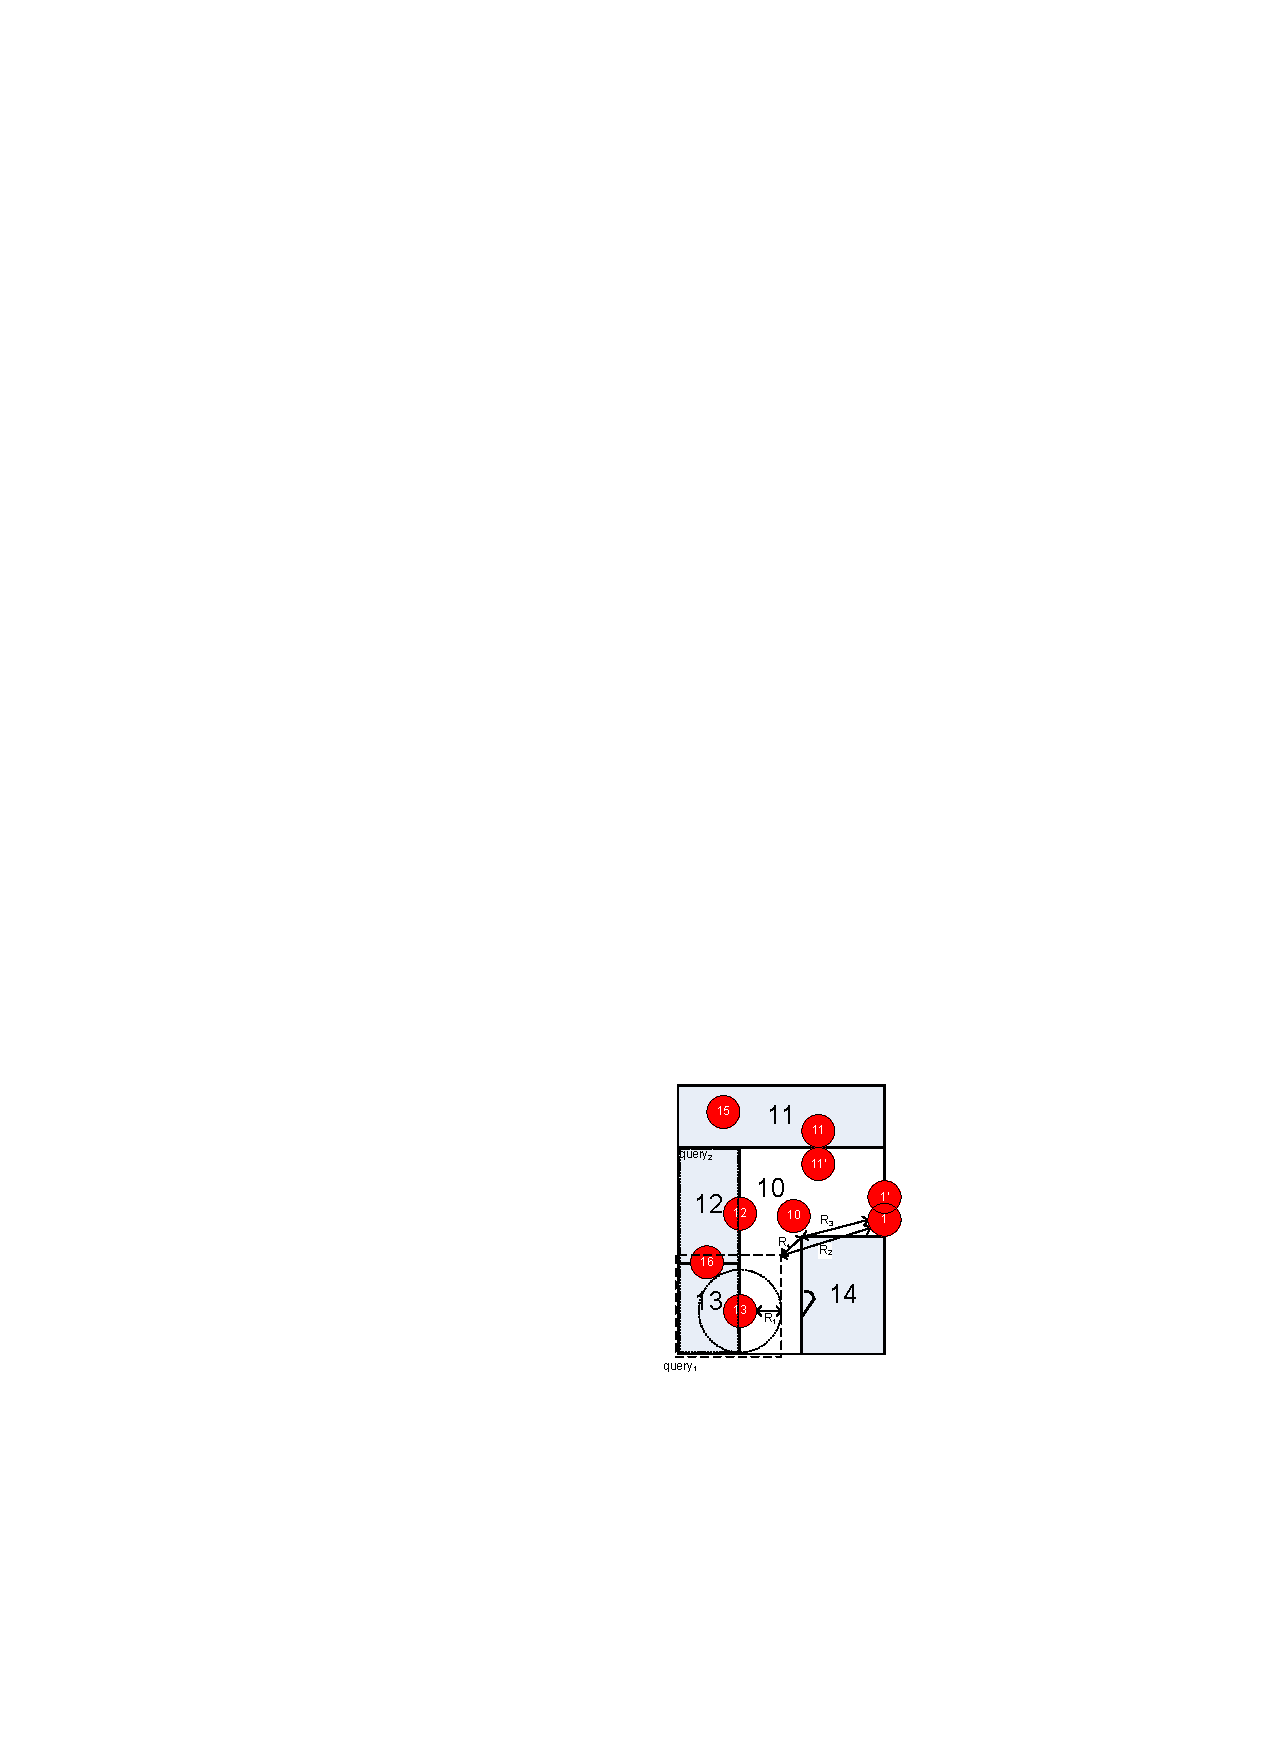
\includegraphics[width=\columnwidth]{figures/2-2/2-2-5.pdf}
    \end{figure}

  \column{.8\textwidth}
    \vspace{-15pt}
    \begin{itemize}
      \ssize{
      \pause
      \item $\mathrm{CLASS1}$ -- \textrm{Device is fully covered in $R$ along with cells, e.g., $(device_{16}, query_2)$}
      \pause
      \item $\mathrm{CLASS2}$ -- \textrm{Device is fully covered but corresponding cells are not,  e.g., $(device_{13}, query_1)$}
      \pause
      \item $\mathrm{CLASS3}$ -- \textrm{Device intersects with the query range $R$,  e.g., $(device_{16}, query_1)$}
      \pause
      \item $\mathrm{CLASS4}$ -- \textrm{Device is disjoint from $R$ and at least one of its corresponding cells in $C_{ic} = \{ c|c \sqcap R \neq \varnothing \}$,  e.g., $(device_{1}, query_1)$}
      \pause
      \item $\mathrm{CLASS5}$ -- \textrm{Device is disjoint from $R$ and at least one of its corresponding cells in $C_{ex} = \{ c| \{ c, c'\} \in G.E, c' \in C_{ic} \}$, but none of them are in $C_{ic}$, e.g., $(device_{10}, query_2)$}
      }
    \end{itemize}

\end{columns}

\end{frame}

%------------------------------------------------

\begin{frame}
\frametitle{Query Registration}

\begin{itemize}
  \item To handle concurrent \textrm{CRMQ}s, a \emph{Query Hash Table} is created hold the results
    \begin{itemize}
      \item $QHT[queryID] = (CR, UR);~ CR \subseteq O_{indoor}, UR \subseteq O_{indoor}$
      \item where $CR$ is the certain result and $UR$ is the uncertain result
    \end{itemize}
  \item Overview
    \begin{figure}[tb]
      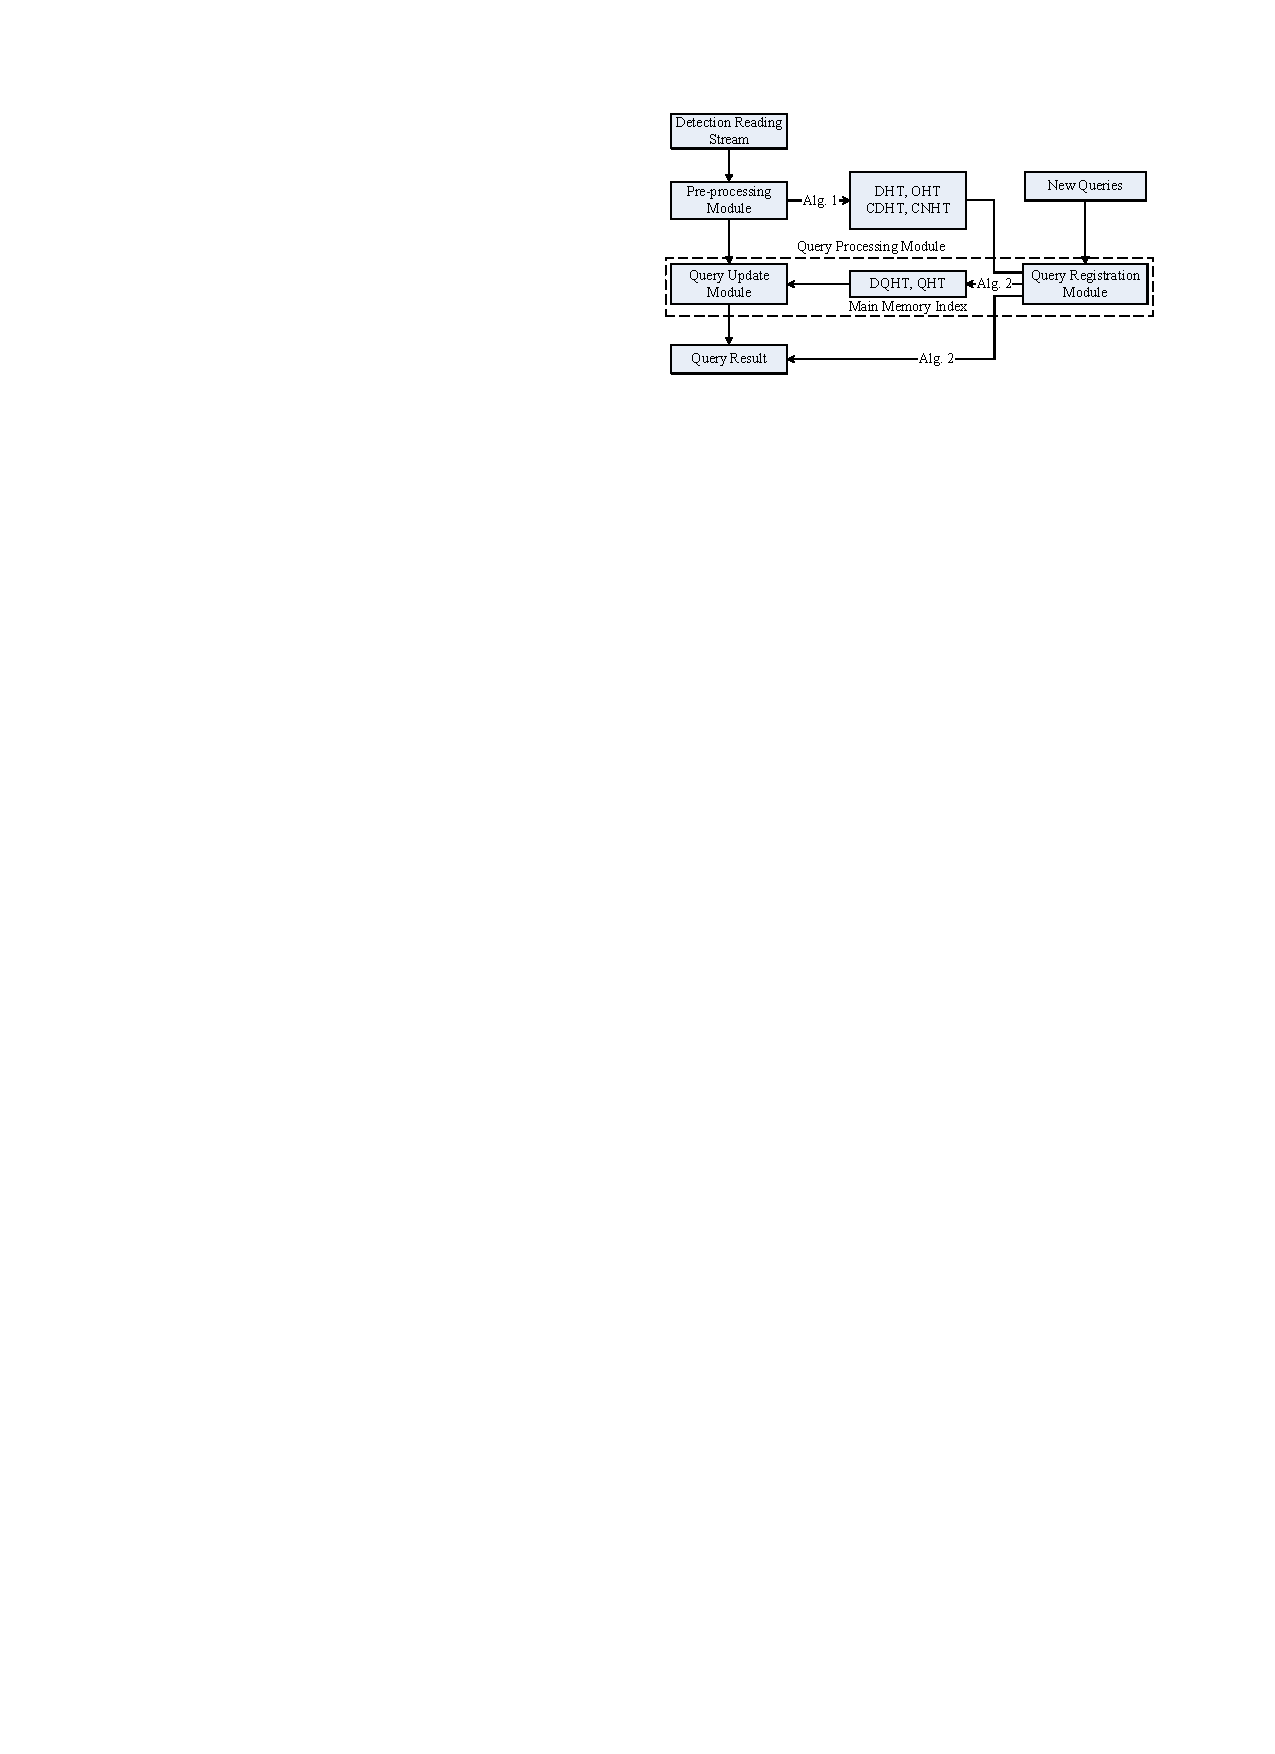
\includegraphics[width=0.68\columnwidth]{figures/2-2/2-2-6.pdf}
    \end{figure}
\end{itemize}

\end{frame}

%------------------------------------------------

\begin{frame}
\frametitle{Query Registration Algorithm (I)}

\begin{columns}[c]

\column{.48\textwidth}
  \begin{figure}[tb]
    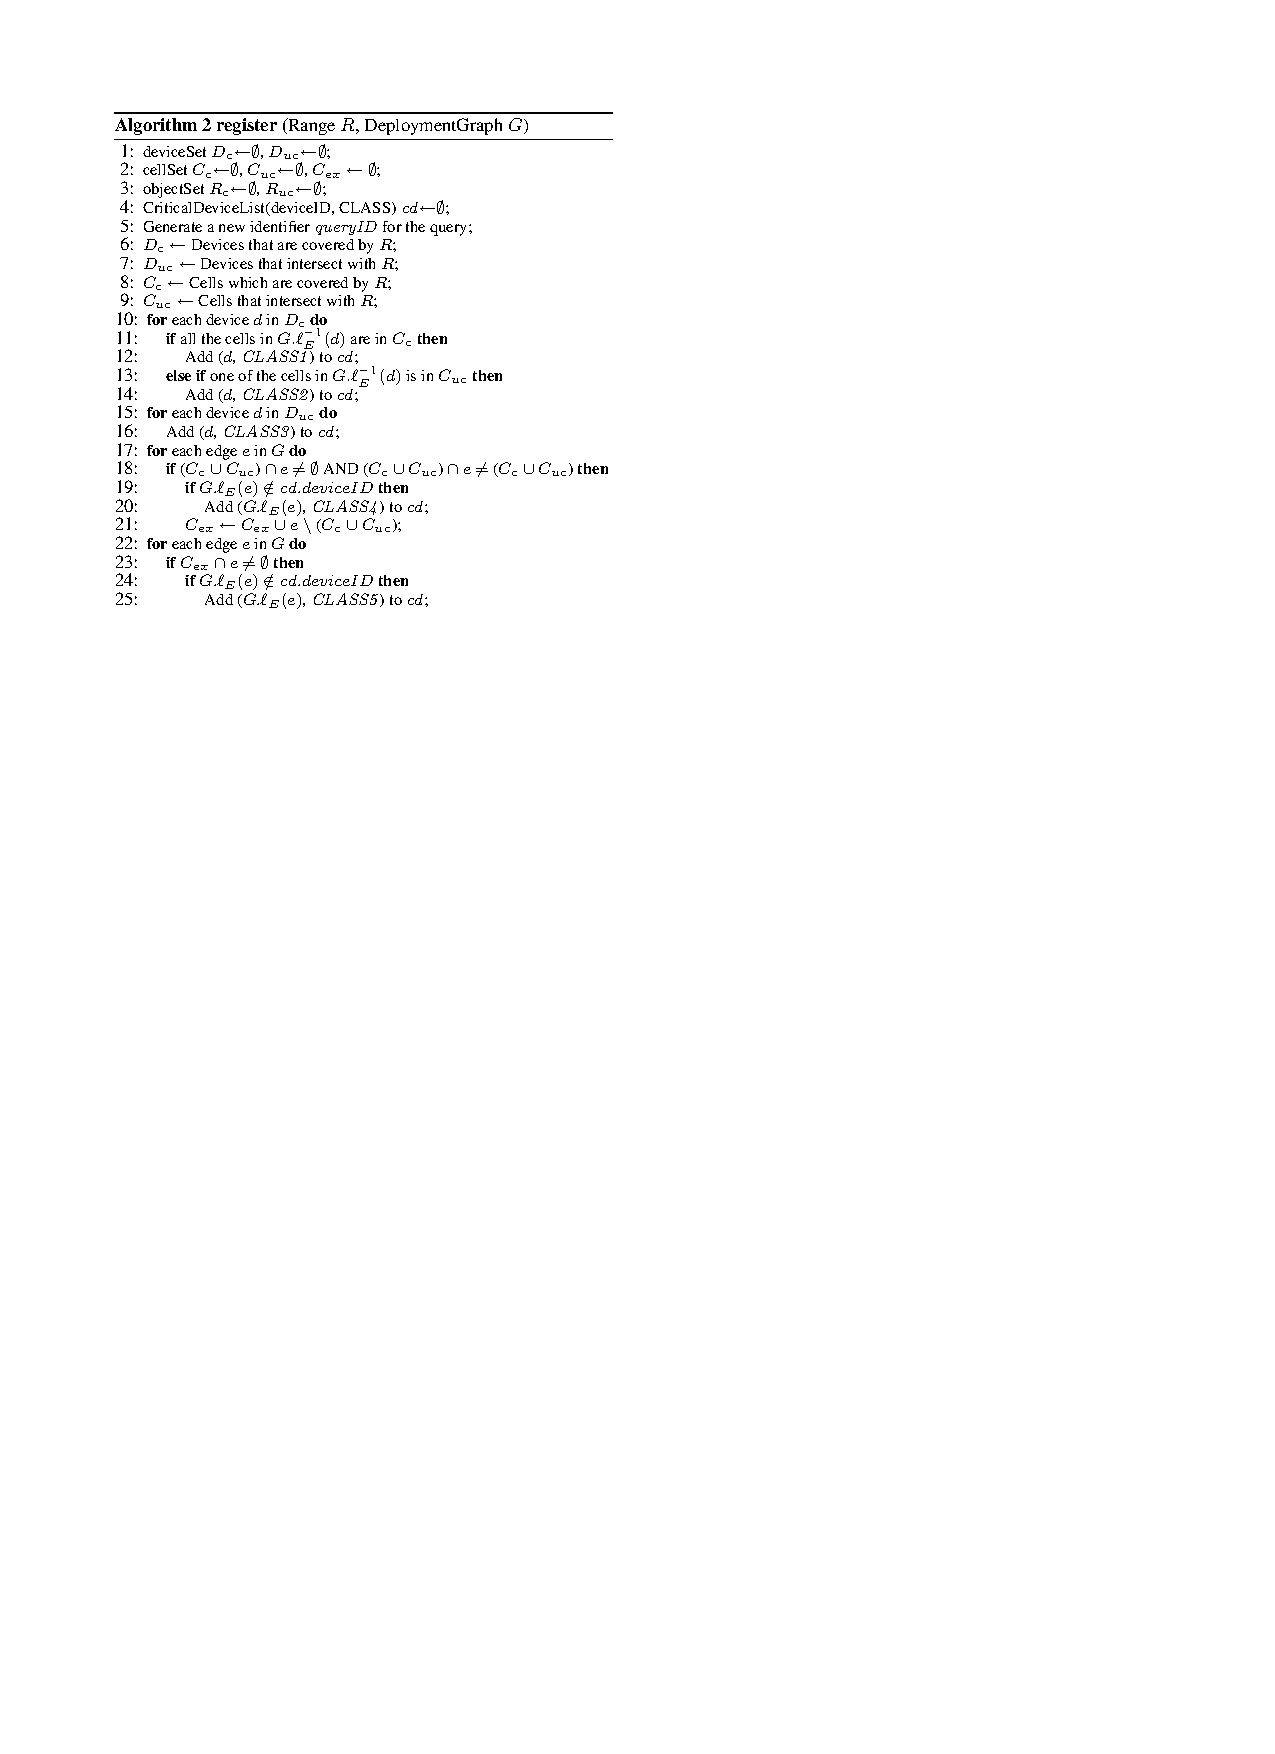
\includegraphics[width=\columnwidth]{figures/2-2/2-2-7.pdf}
  \end{figure}

\column{.6\textwidth}
\ssize{
  \begin{enumerate}
    \pause
    \item Lines 1--9: \textrm{Initialization} \pause
    \item Lines 10--14: \textrm{Add possible devices to CriticalDeviceList $cd$ ($\mathrm{CLASS1}$ and $\mathrm{CLASS2}$)} \pause
    \item Lines 15--16: \textrm{Add possible $\mathrm{CLASS3}$ devices} \pause
    \item Lines 17--20: \textrm{Add possible $\mathrm{CLASS4}$ devices} \pause
    \item Line 21: \textrm{Determine extended cell set $C_{ex}$} \pause
    \item Lines 22--25: \textrm{Add possible $\mathrm{CLASS5}$ devices}
  \end{enumerate}
}
\end{columns}

\end{frame}

%------------------------------------------------

\begin{frame}
\frametitle{Query Registration Algorithm (II)}

\begin{columns}[c]

\column{.48\textwidth}
  \begin{figure}[tb]
    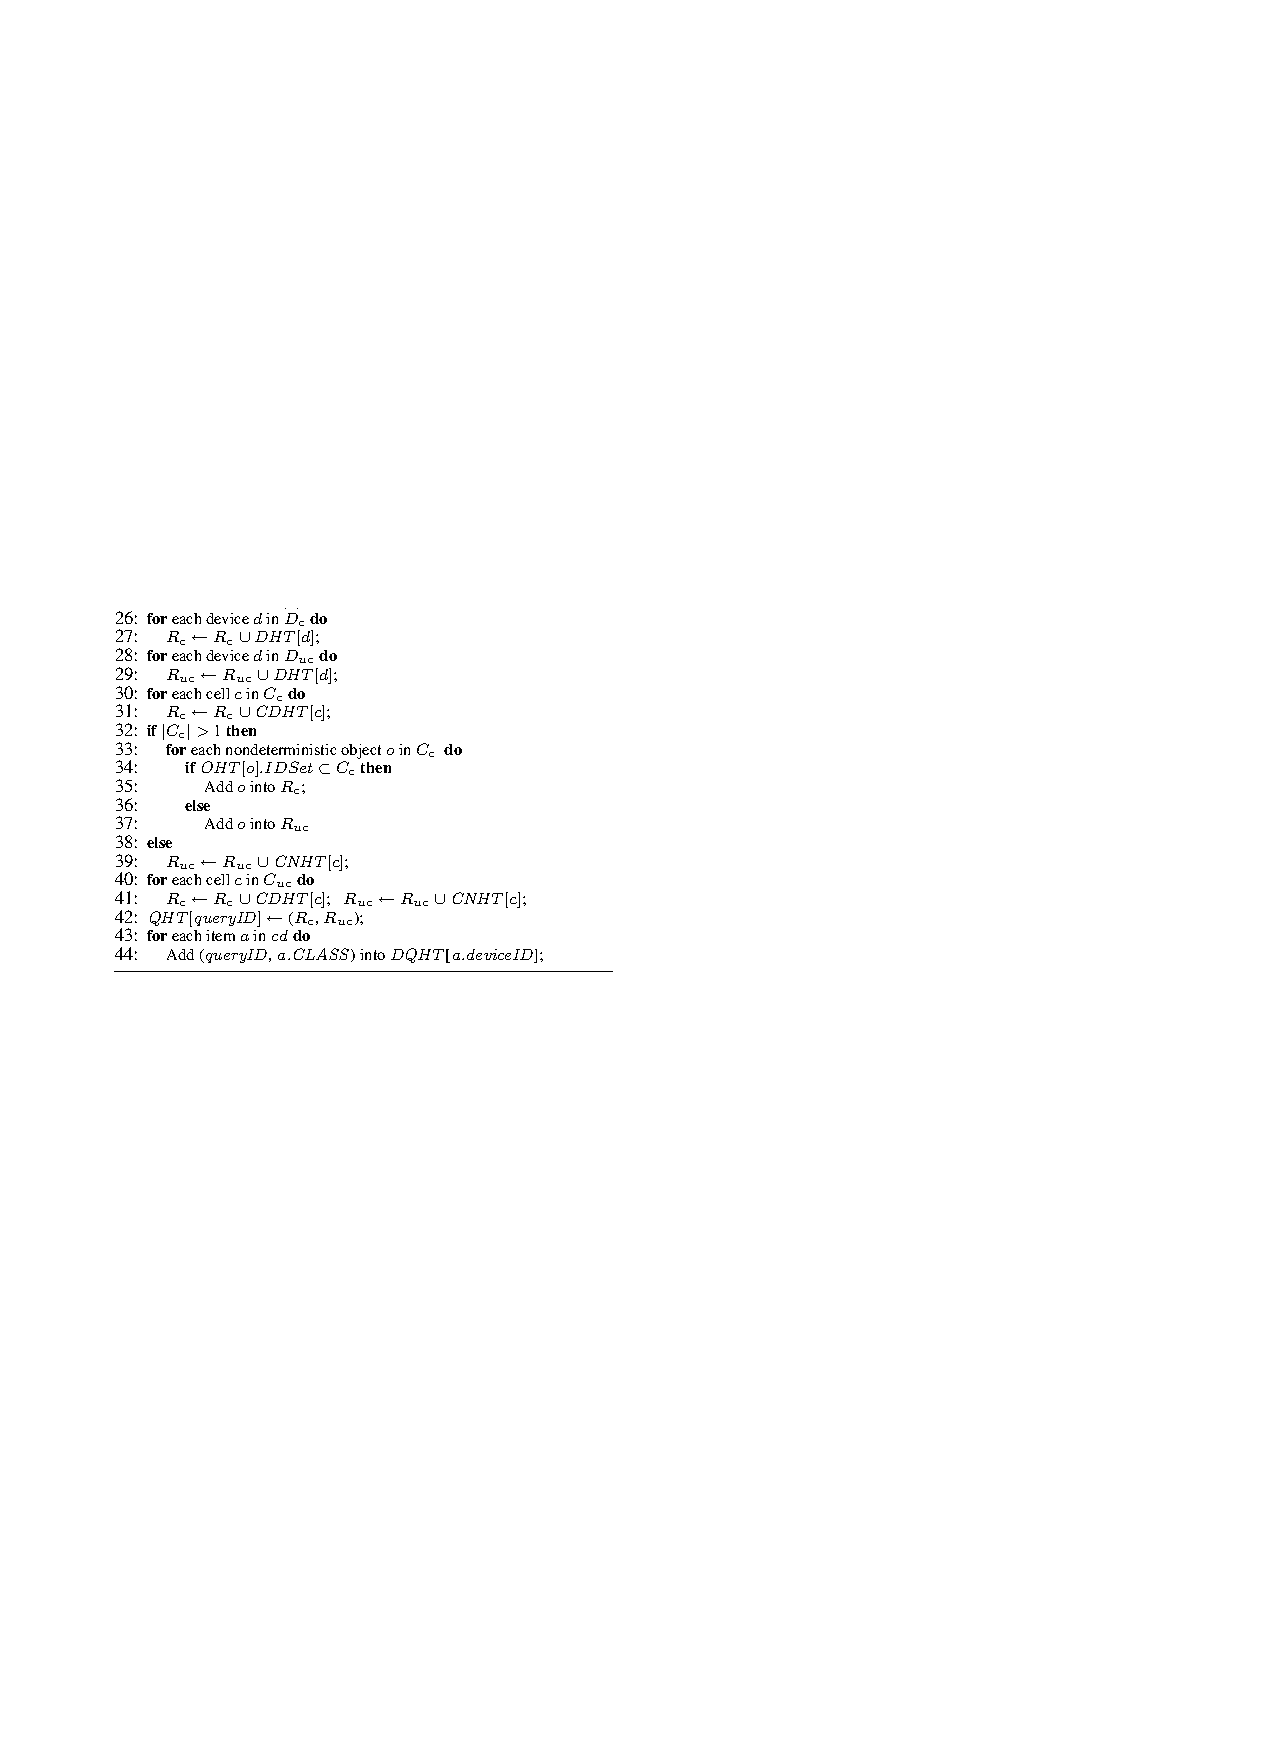
\includegraphics[width=\columnwidth]{figures/2-2/2-2-8.pdf}
  \end{figure}

\column{.6\textwidth}
\vspace{-10pt}
\ssize{
  \begin{enumerate}
    \pause
    \item Lines 26--27: \textrm{Add active objects from DHT to the certain result} \pause
    \item Lines 28--29: \textrm{Intersected device set, add active objects from DHT to the uncertain result} \pause
    \item Lines 30--31: \textrm{From covered cells, add deterministic objects to the certain result} \pause
    \item Lines 32-37: \textrm{If more than one cell, check nondeterministic objects. If all its possible cells are in $C_c$ add the object to the certain result, else uncertain result} \pause
    \item Lines 38--39: \textrm{Only one cell. Nondeterministic objects are added to the uncertain result} \pause
    \item Lines 40--41: \textrm{Intersected set. Add all objects to the uncertain result} \pause
    \item Line 42: \textrm{Results added to QHT} \pause
    \item Lines 43--44: \textrm{DQHT entry is created for each critical device}
  \end{enumerate}
}
\end{columns}

\end{frame}

%------------------------------------------------

\begin{frame}
\frametitle{Query Result Updates}

\begin{itemize}
  \fsize{
  \item When an object enters the activation range of a critical device:
    \begin{itemize}
      \ssize{
      \item For $\mathrm{CLASS1}$ or $\mathrm{CLASS2}$ devices the object is the certain result
      \item For $\mathrm{CLASS3}$ devices the object is possibly in the query range
      \item For $\mathrm{CLASS4}$ or $\mathrm{CLASS5}$ devices the object is not in the query range
      }
    \end{itemize}
  \item When an object leaves:
    \begin{itemize}
      \ssize{
      \item For $\mathrm{CLASS1,3,5}$ devices there are no changes
      \item For $\mathrm{CLASS2}$ devices the object may still be in the query range, thus it is moved to the uncertain result
      \item For $\mathrm{CLASS4}$ devices the object may be in a cell that intersects with the query range and it added to the uncertain result
      }
    \end{itemize}
  }
\end{itemize}

\begin{figure}[tb]
  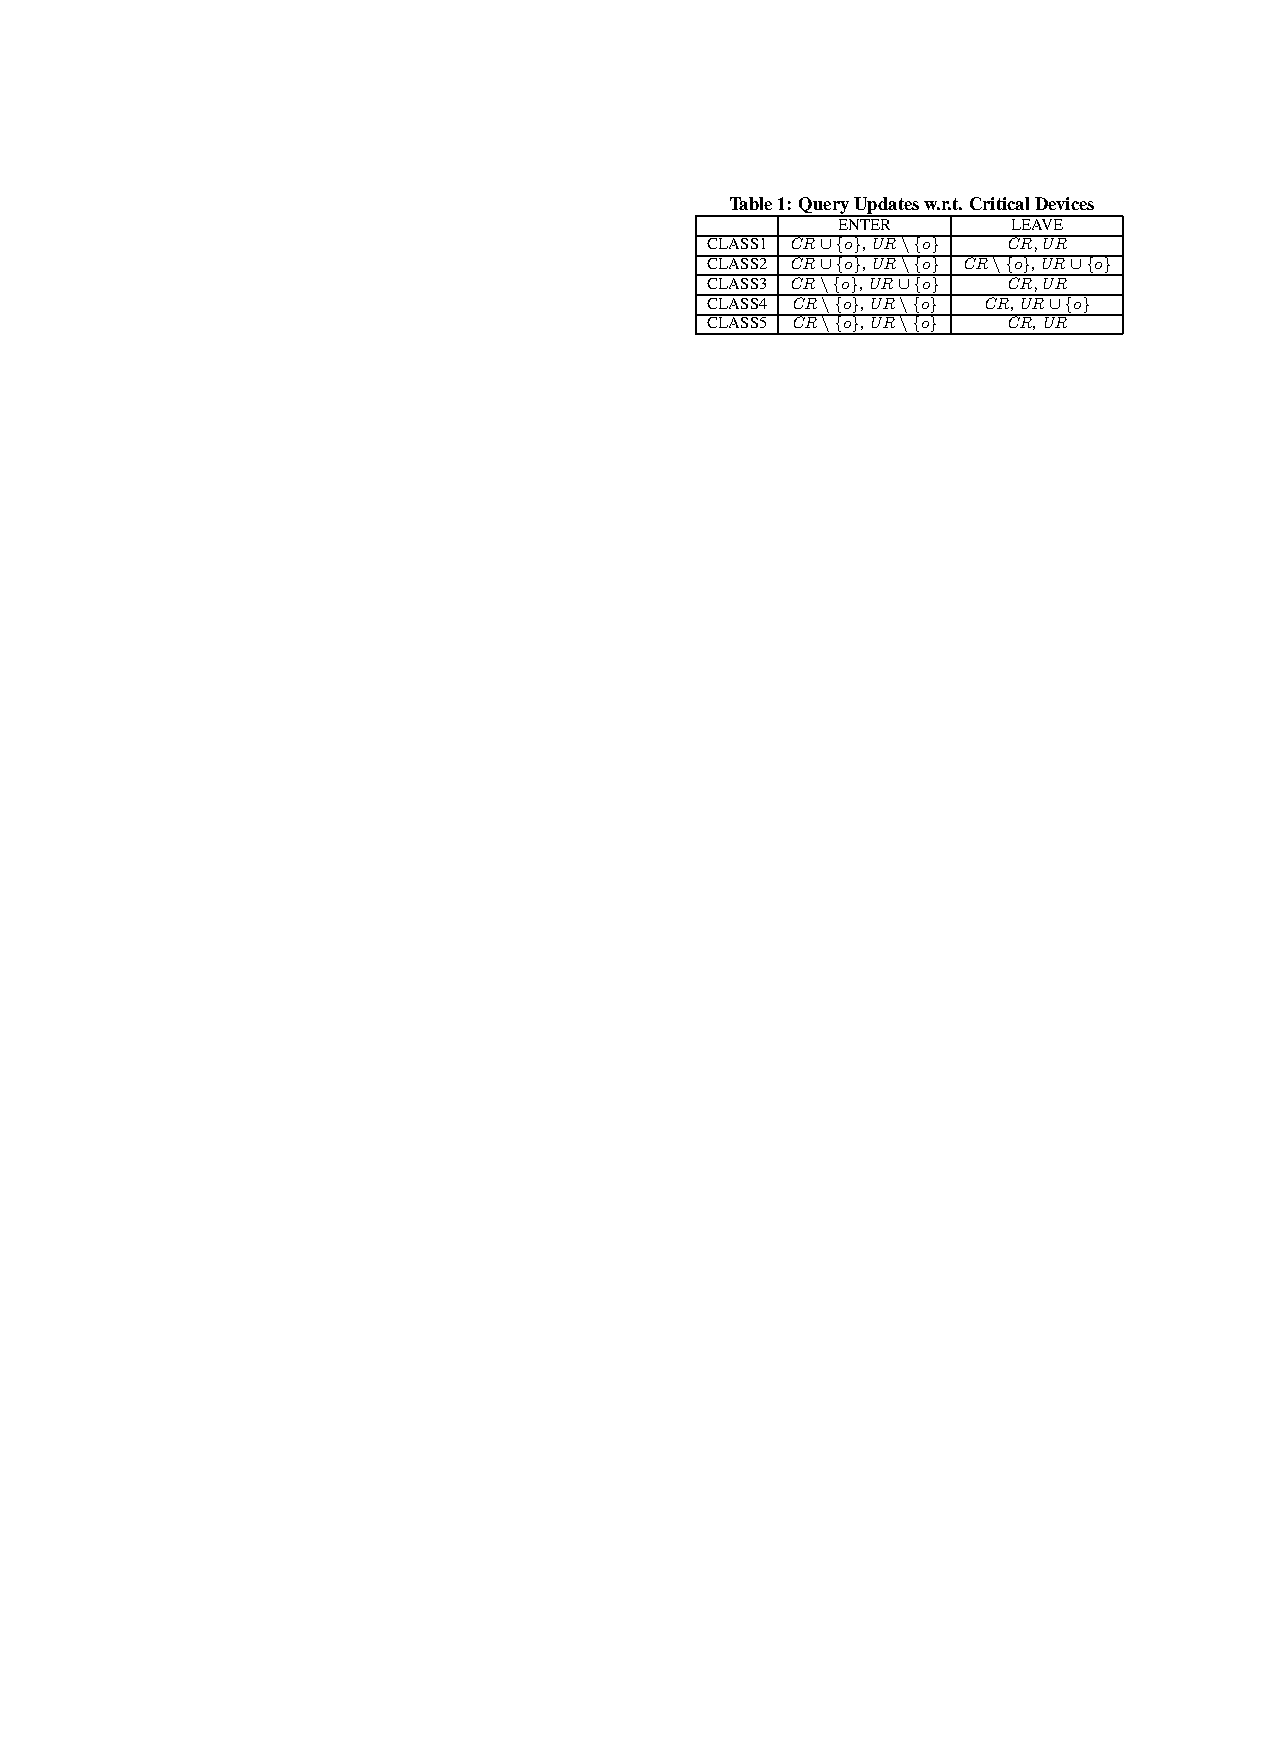
\includegraphics[width=0.75\columnwidth]{figures/2-2/2-2-9.pdf}
\end{figure}

\end{frame}

%------------------------------------------------

\begin{frame}
\frametitle{Deferred Query Updates}

\begin{itemize}
	\item Deferred query updates is the concept of postponing updates where we already know the result
  \item The time a query result is still valid is calculated from \emph{minimum indoor walking distance} divided by the \emph{maximum speed} an object can travel
\end{itemize}

\begin{columns}[c]

\column{.3\textwidth}
  \begin{figure}[tb]
    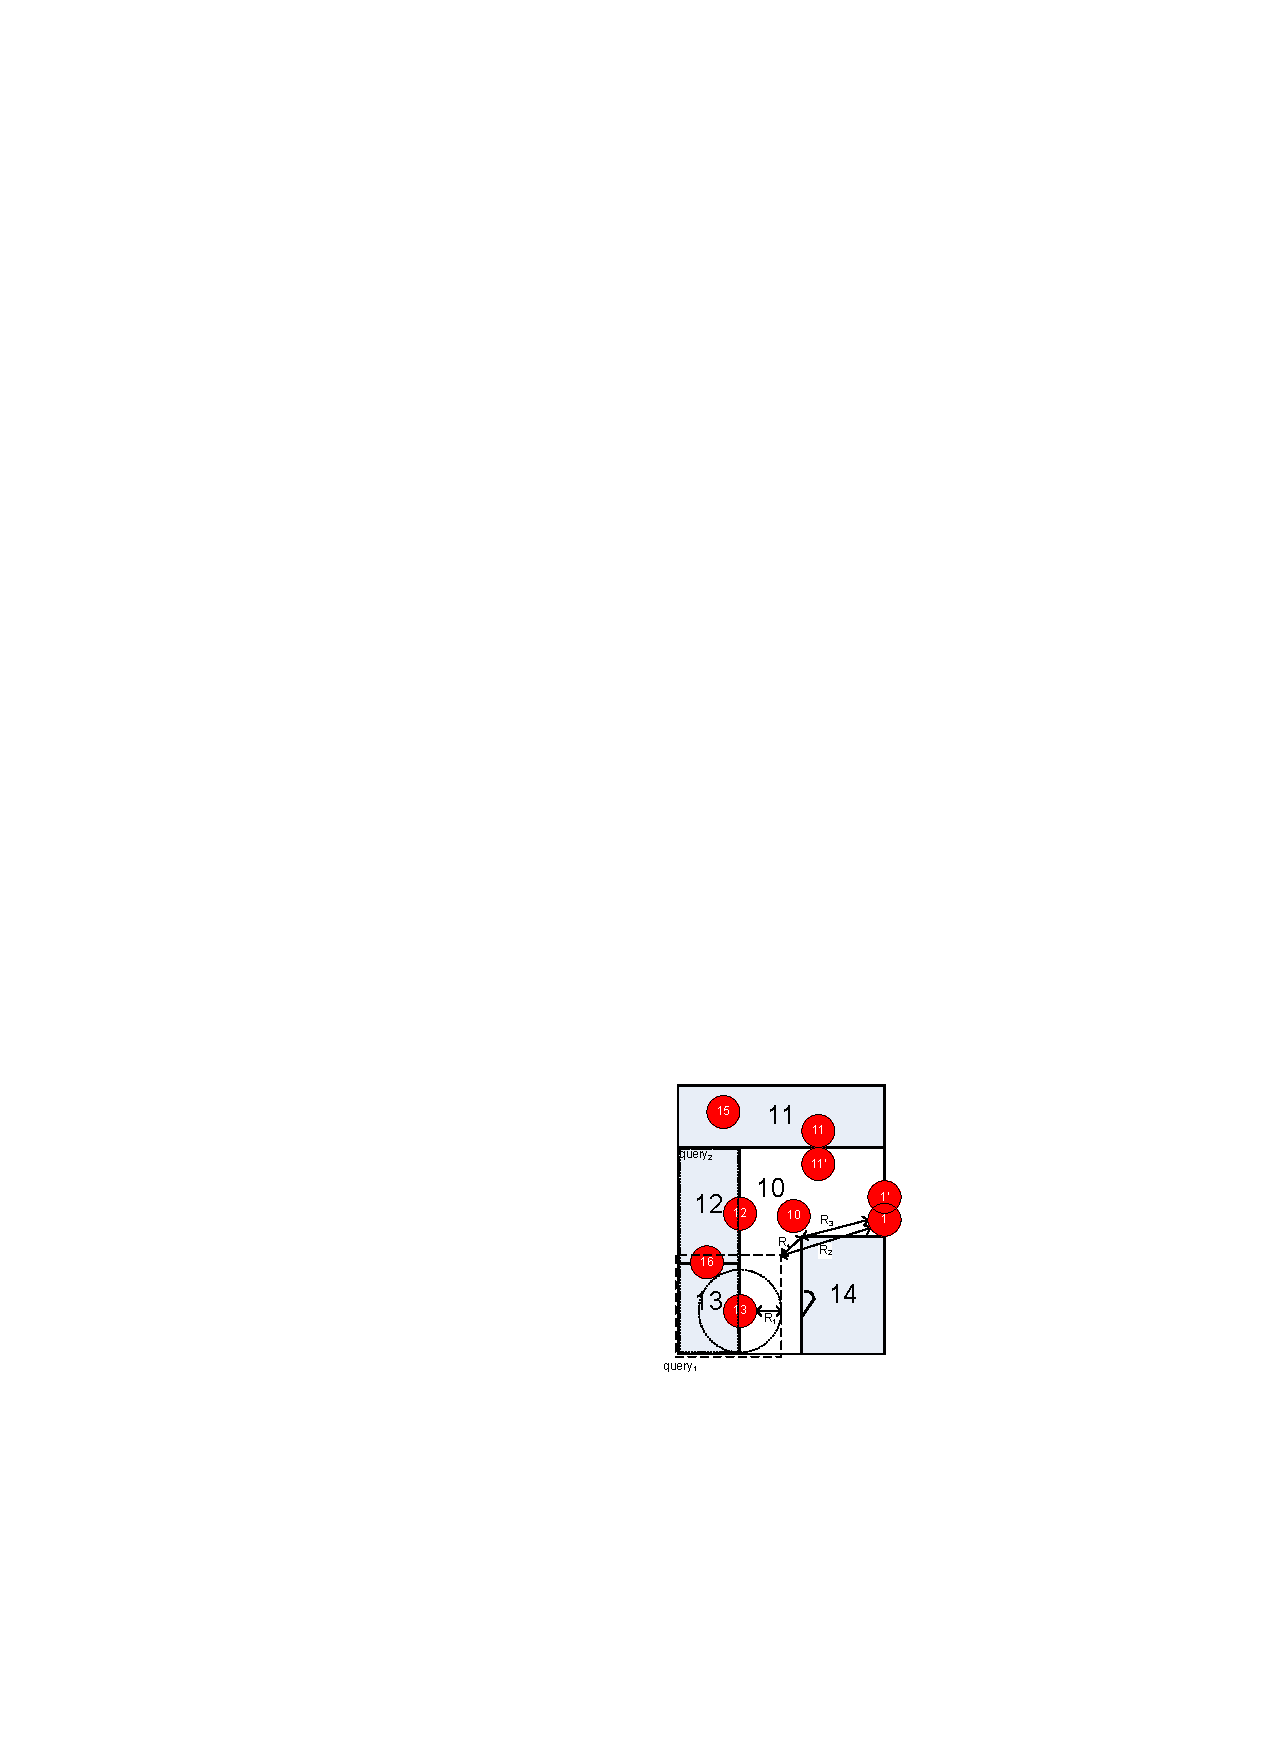
\includegraphics[width=\columnwidth]{figures/2-2/2-2-5.pdf}
  \end{figure}

\column{.7\textwidth}
  \fsize{
  Consider $query_1$, after the object $o$ leaves a $\mathrm{CLASS2}$ critical device $devoce_{13}$, it should be moved from certain to uncertain result.
  \\~\\
  Let $V_{max}$ be the maximum speed, if $R_1 = V_{max} * \Delta t$, the certain result can be maintained without updating for an extra period of time $\Delta t$.
  }
\end{columns}

\end{frame}

%------------------------------------------------

\begin{frame}
\frametitle{Deferred Query Updates}

\begin{itemize}
	\item Deferred query updates is the concept of postponing updates where we already know the result
  \item The time a query result is still valid is calculated from \emph{minimum indoor walking distance} divided by the \emph{maximum speed} an object can travel
\end{itemize}

\begin{columns}[c]

\column{.3\textwidth}
  \begin{figure}[tb]
    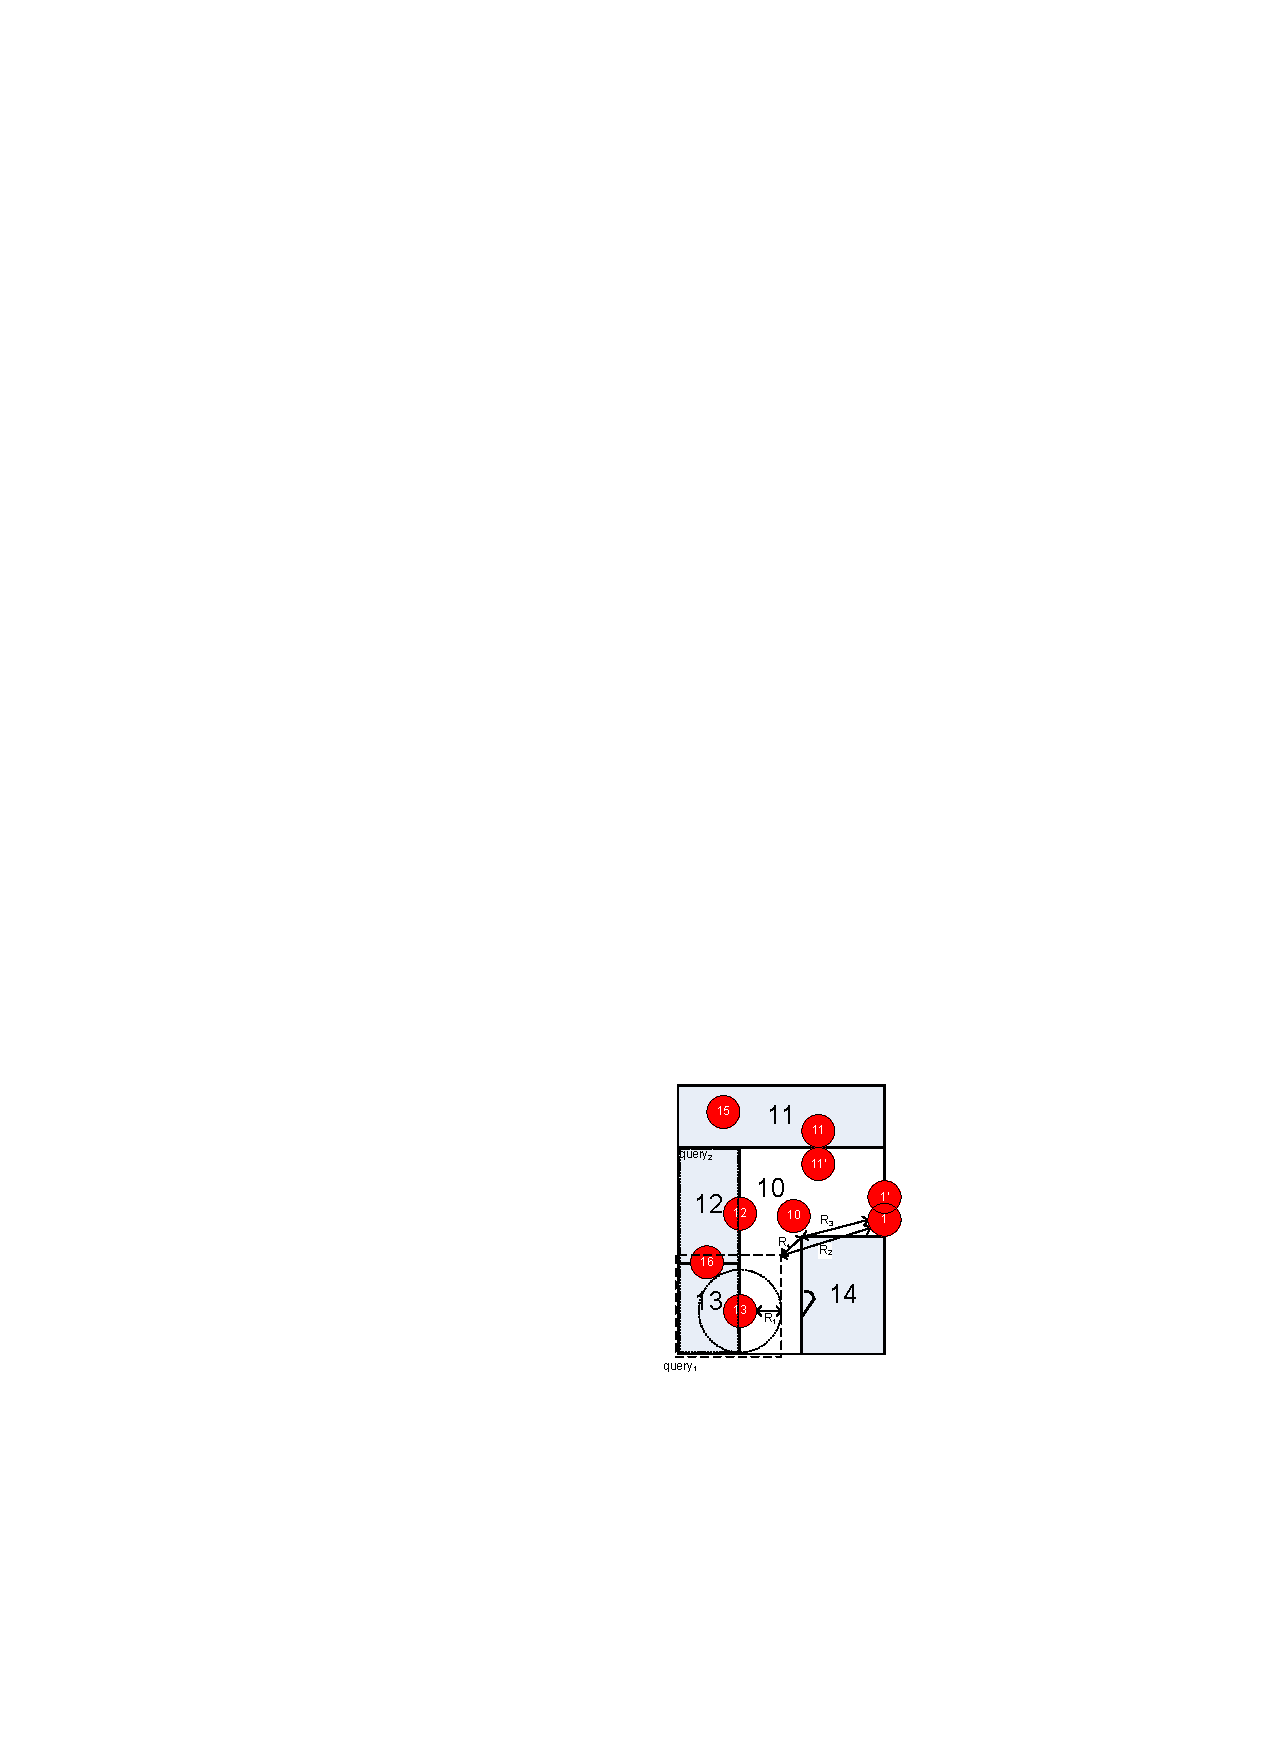
\includegraphics[width=\columnwidth]{figures/2-2/2-2-5.pdf}
  \end{figure}

\column{.7\textwidth}
  \fsize{
  Consider $query_1$, after the object $o$ leaves a $\mathrm{CLASS2}$ critical device $devoce_{13}$, it should be moved from certain to uncertain result.
  \\~\\
  Let $V_{max}$ be the maximum speed, if $R_1 = V_{max} * \Delta t$, the certain result can be maintained without updating for an extra period of time $\Delta t$.
  }
\end{columns}

\end{frame}

%------------------------------------------------

\begin{frame}
\frametitle{Probabilistic Analysis of Uncertain Results}

\fsize{\textrm{
To analyze probability that $o$ is in the query range $R$. Assume that the possible locations in a given indoor space conform a uniform distribution within all reachable regions constrained by its maximum speed.
}}
\\~\\
\textit{1. Probabilities for Active Objects}
\\~\\
Formally, the probability that an active object $o$ is in the range $R$ is defined as:

\begin{equation}
  prob(o \Theta R) = \frac{Area(Devices(d).ActRange \sqcap R)}{Area(Devices(d).ActRange)}
\end{equation}

\begin{columns}[c]

\column{.3\textwidth}
  \vspace{-15pt}
  \begin{figure}[tb]
    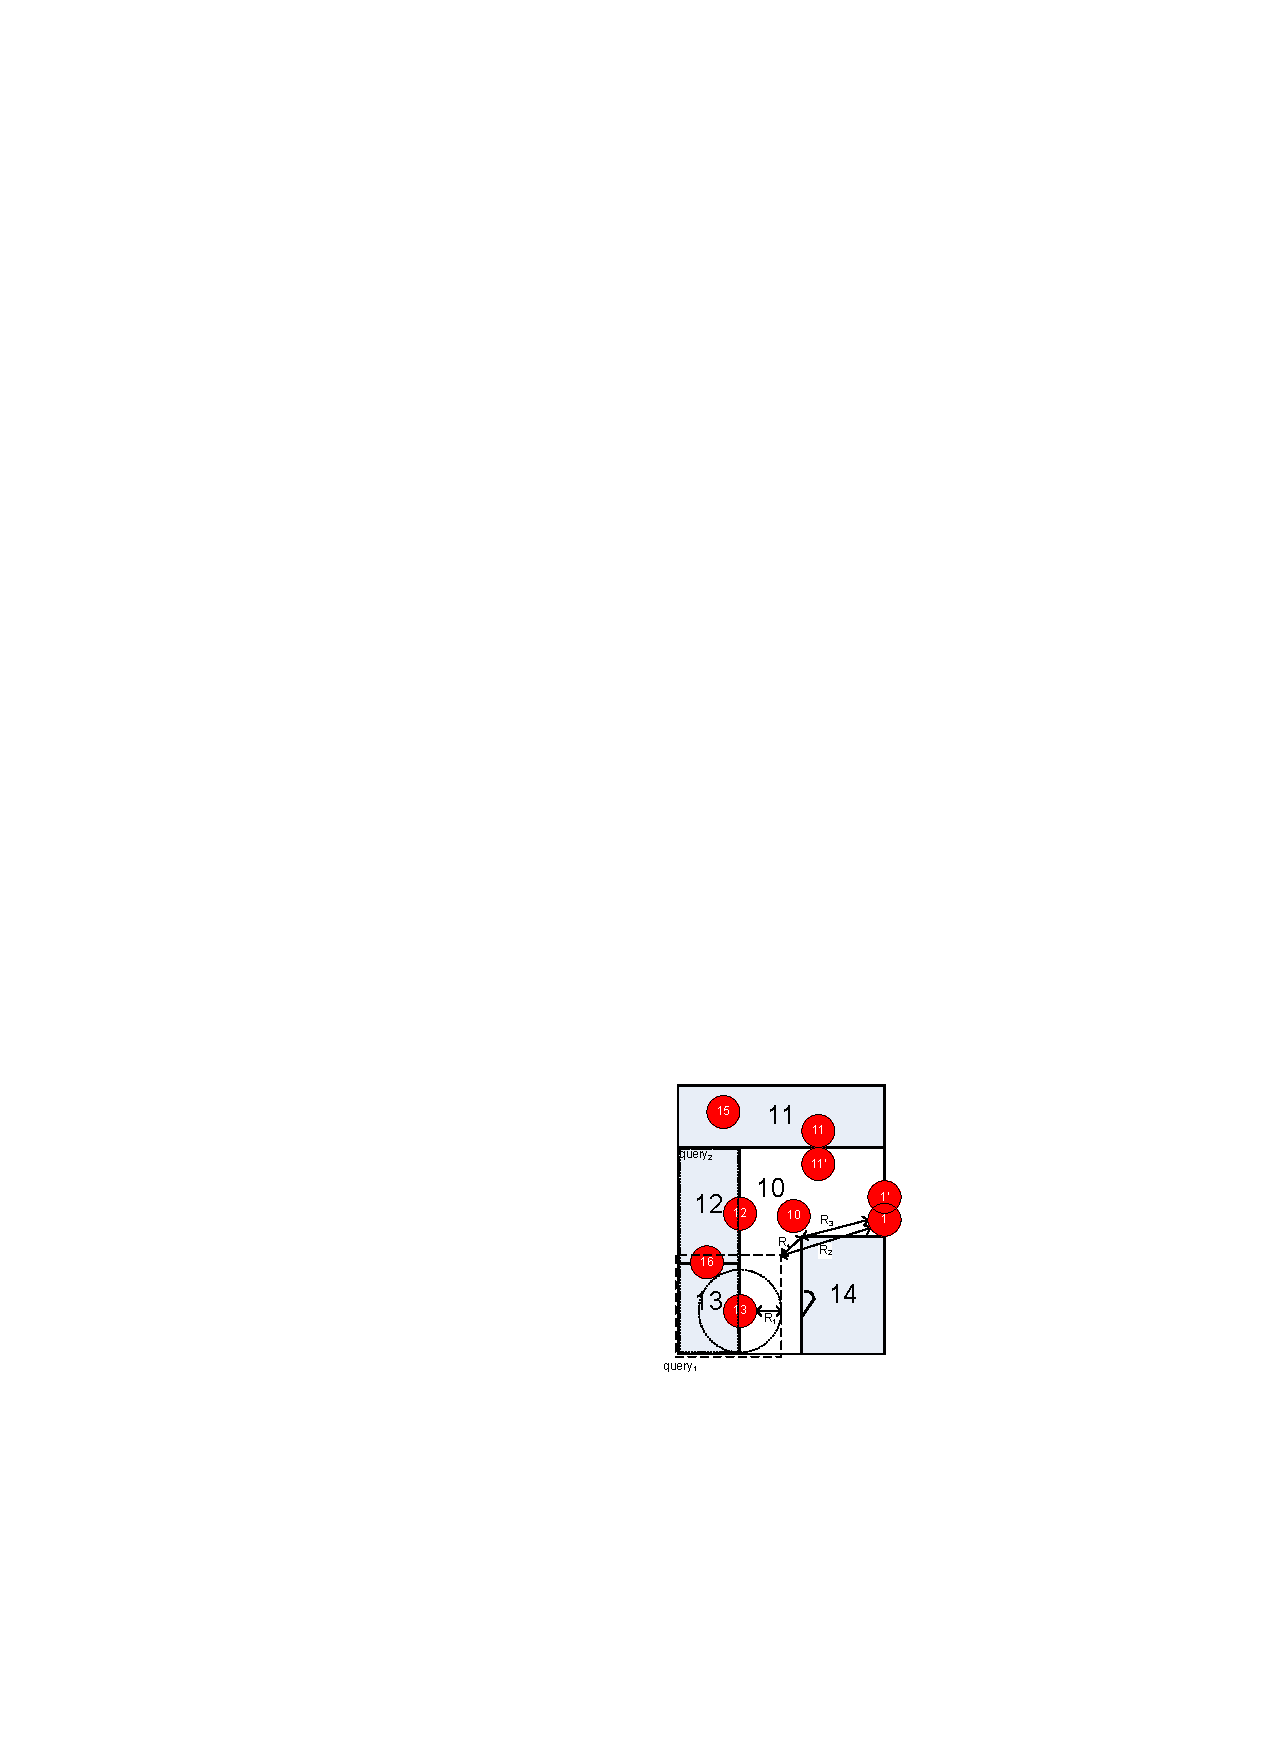
\includegraphics[width=\columnwidth]{figures/2-2/2-2-5.pdf}
  \end{figure}

\column{.7\textwidth}
  Consider $device_{16}$, a $\mathrm{CLASS3}$ device for $query_1$, the probability for an active object in $device_{16}$ to be in the query range is calculated as ...

\end{columns}

\end{frame}

%------------------------------------------------

\begin{frame}
\frametitle{Probabilistic Analysis of Uncertain Results}

\textit{2. Probabilities for Inactive Objects}
\\~\\
For the case that after leaving $\mathrm{CLASS2,3,4}$ devices, the probabilities for inactive objects can be defined based on the maximum speed constraint.
\\~\\
An example for an inactive object that just leaves $device_{12}$...
\vspace{-5pt}
\begin{figure}[tb]
  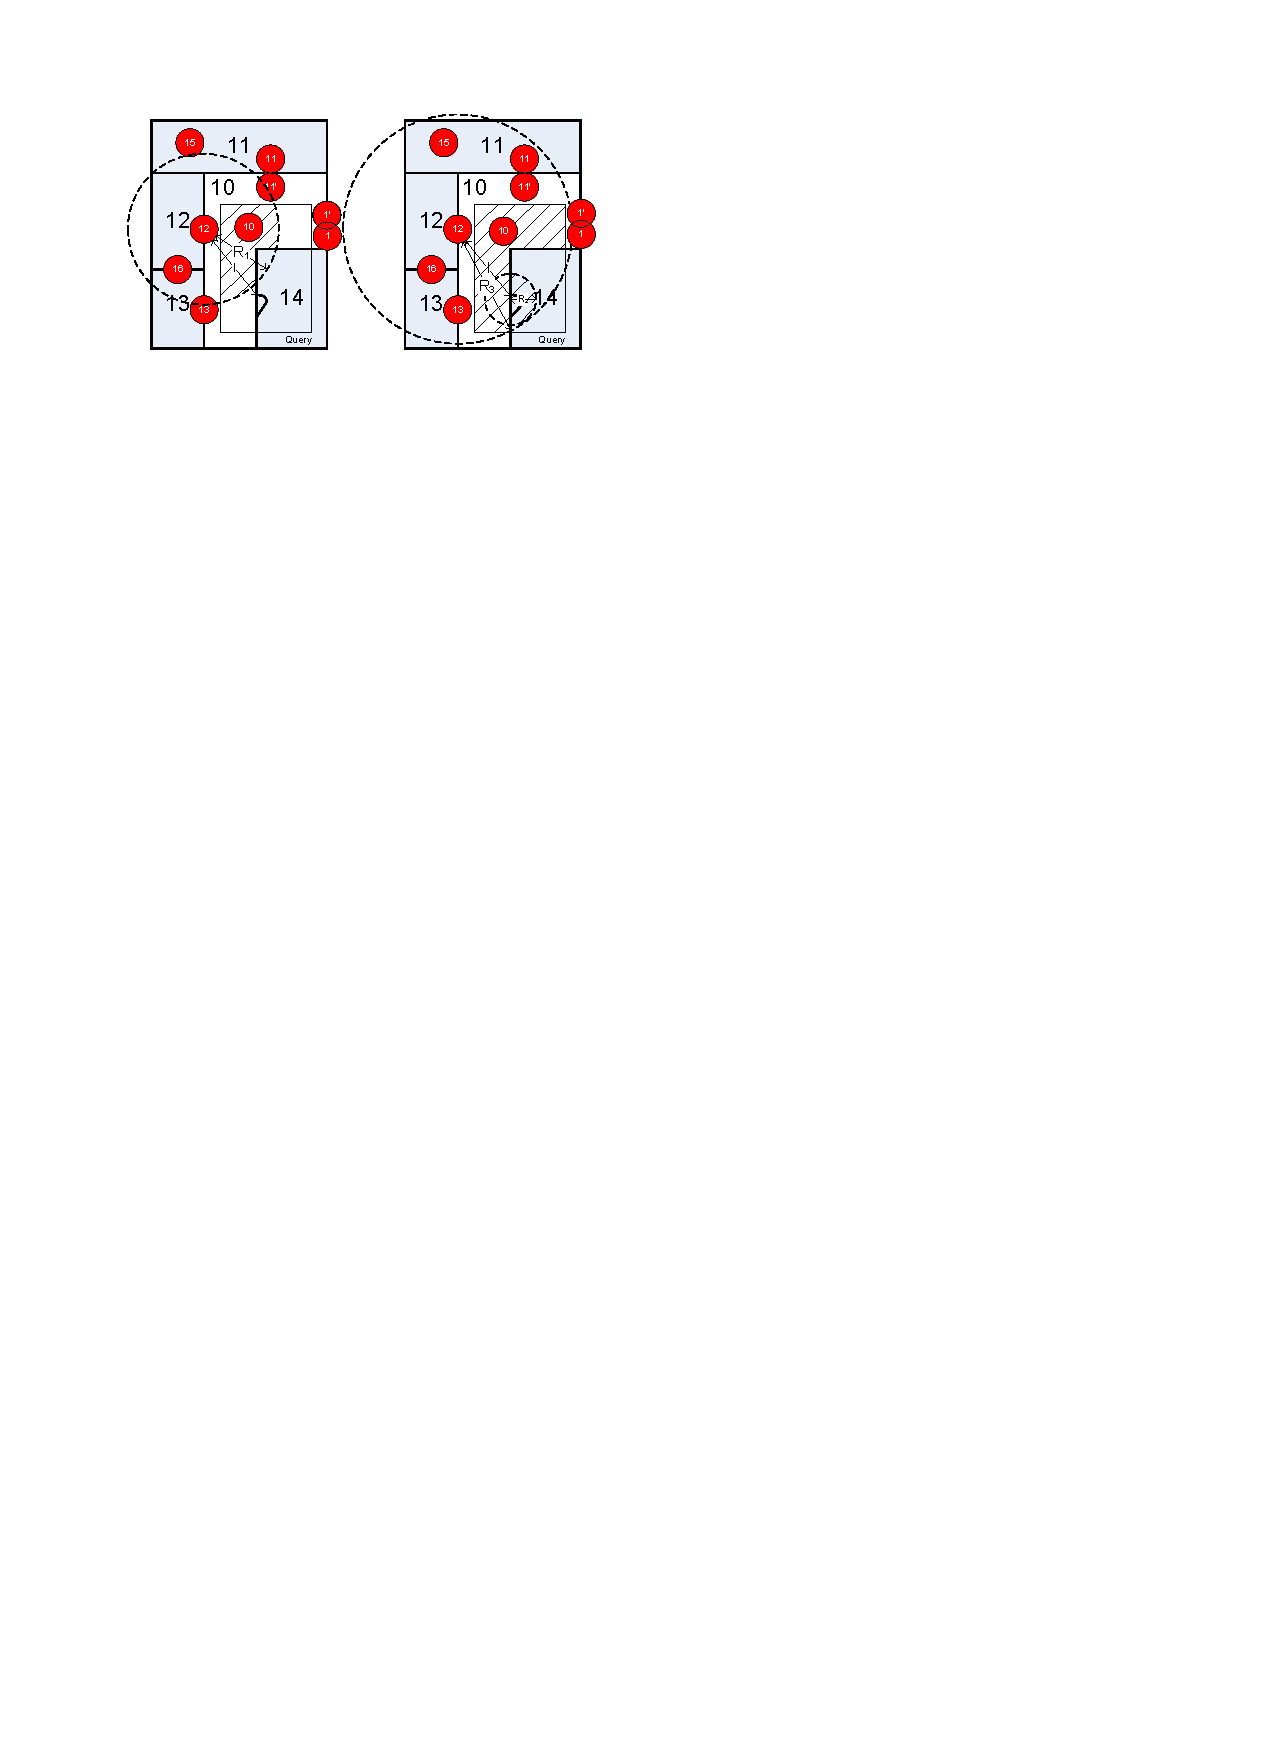
\includegraphics[width=0.7\columnwidth]{figures/2-2/2-2-10.pdf}
\end{figure}

\end{frame}

%------------------------------------------------

\begin{frame}
\frametitle{Conclusion}

\begin{itemize}
	\item A solution with a symbolic model of the floor plan, device locations, and activation ranges
  \item Data is stored in several hash tables which make it possible to efficiently locate a specific object (result is a signle room/cell, or a set of rooms/cells)
  \item Future work
    \begin{itemize}
      \item sharing of query processing among concurrent queries
      \item common critical devices exploitation
      \item other types of queries: range and $k$NN
      \item further investigate the probability analysis
    \end{itemize}
\end{itemize}

\end{frame}
